\subsection{\texorpdfstring{$y''+(ax^4+bx^3+cx^2+dx+e)y = 
0$}{y''-(ax4+bx3+cx2+dx+e)y = 0}}

Auch ein Polynom $4$-ten Grades stellt kein Problem mehr dar. In die 
Formel (\ref{eq:wellen:allgemeineak}) eingesetzt, ergibt

\begin{equation*}
	\begin{split}
		a_k &= -\frac{1}{k(k-1)} (aa_{k-2-4} + 
		ba_{k-2-3} + ca_{k-2-2} + da_{k-2-1} +ea_{k-2-0})
		\\
		&= -\frac{1}{k(k-1)} (aa_{k-6} + ba_{k-5} + 
		ca_{k-4} + da_{k-3} +ea_{k-2}), \qquad a_{k<0} = 0
	\end{split}
\end{equation*}

Vergleichen wir die zwei Wellen, die bei dem Polynom 2-ten und bei dem 
4-ten Grades entstehen (Abbildung \ref{fig:wellen:poly4-dgl}), kann man sehen, 
dass im Bereich, wo sich die Profile $p(x)$ "uberlagern, auch die Wellen 
konvergent sind. Der Unterschied liegt darin, dass die Schwingung des Polynomes 
2-ten Grades nicht mehr zur"uckkommt und exponentiell verl"auft, da die Parabel 
keine weiteren Nullstellen mehr besitzt. Die Schwingung des Polynomes 4-ten 
Grades kommt am Rand der Abbildung zur"uck, sie wird also vom Polynom nochmal 
nach unten gezogen und wechselt ihren Verlauf bei der Nullstelle noch einmal, 
was somit unsere Erkenntnisse best"atigt. 

\begin{figure}
	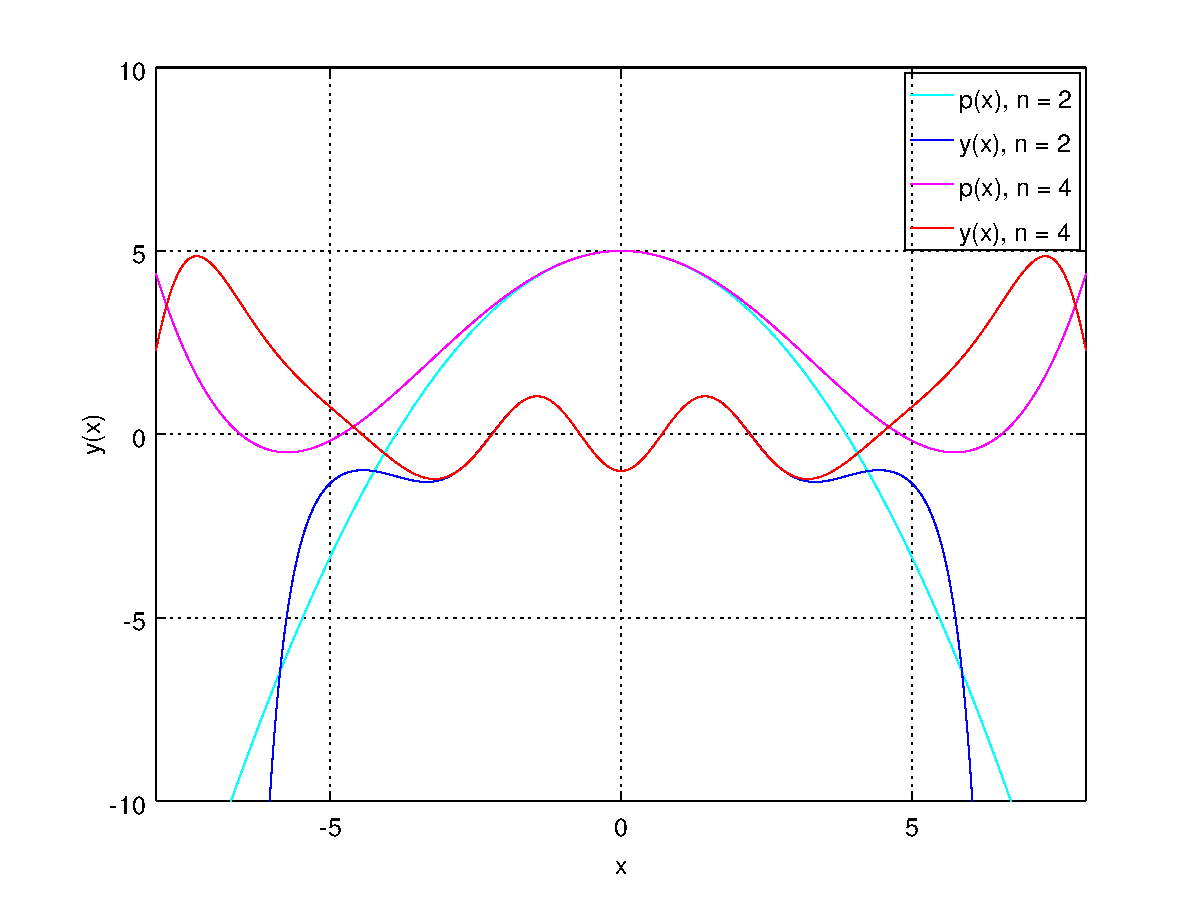
\includegraphics[scale=0.65]{./wellen/images/allgemein/n4.pdf}
	\caption{Vergleich Polynom 2-ten und 4-ten Grades}
	\label{fig:wellen:poly4-dgl}
\end{figure}